El componente utilizado para ampliar la señal enviada por el Arduino al motor, sirviendo de intermediario entre éste y los motores es el módulo específico para el control mediante PWM de motores con un circuito integrado LMD18200T que soporta hasta tres Amperios. En definitiva es un puente H controlado por PWM.\\

Ha sido elegido por satisfacer todas los requisitos necesarios en nuestra tarea: Precio, voltaje, amperaje y de implementación sencilla. Este módulo podría fabricarse, dado su sencillez, a mano comprando los componentes por separado, sin demasiado esfuerzo.\\
\begin{figure}[H]
		\centering
		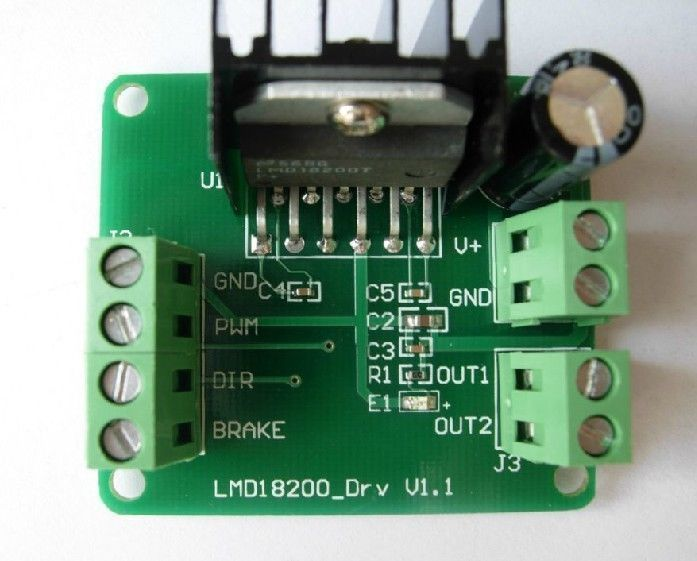
\includegraphics[scale = 0.3]{part/Proyecto_ejecutivo/memoria_constructiva/motor/img/modulopot}
		\caption[Módulo de potencia.]{Módulo de potencia.\\Fuente: \url{http://i.ebayimg.com/}(2014)}\label{fig:figure}
\end{figure}
	
Se aprecian en la figura 6 las entradas y las salidas de las que dispone. De arriba abajo la primera columna es de entradas:

\begin{itemize}
	\item \textbf{GND:} La tierra de la placa de control, en nuestro caso el Arduino.
	\item \textbf{PWM(Pulse width modulation):} la señal del control por ancho de pulsos.
	\item \textbf{Dir:} Señal con el sentido de giro que se desea.
	\item \textbf{Brake:} Freno del motor
\end{itemize}

Y la segunda columna de alimentación y salidas:

\begin{itemize}
	\item \textbf{V+:} Alimentación de 12 voltios.
	\item \textbf{GND:} tierra.
	\item \textbf{OUT1:} Salida de una mitad del puente H.
	\item \textbf{OUT2:} Salida de la otra mitad del puente H
\end{itemize}

La composición del circuito conocido como puente H y su implementación en este módulo viene detallada en el ANEXO donde se referencia al manual del circuito integrado.

		\textbf{Conexión}
El esquema de conexión hacia los elementos con los que interactúa es el siguiente:
\begin{figure}[H]
		\centering
		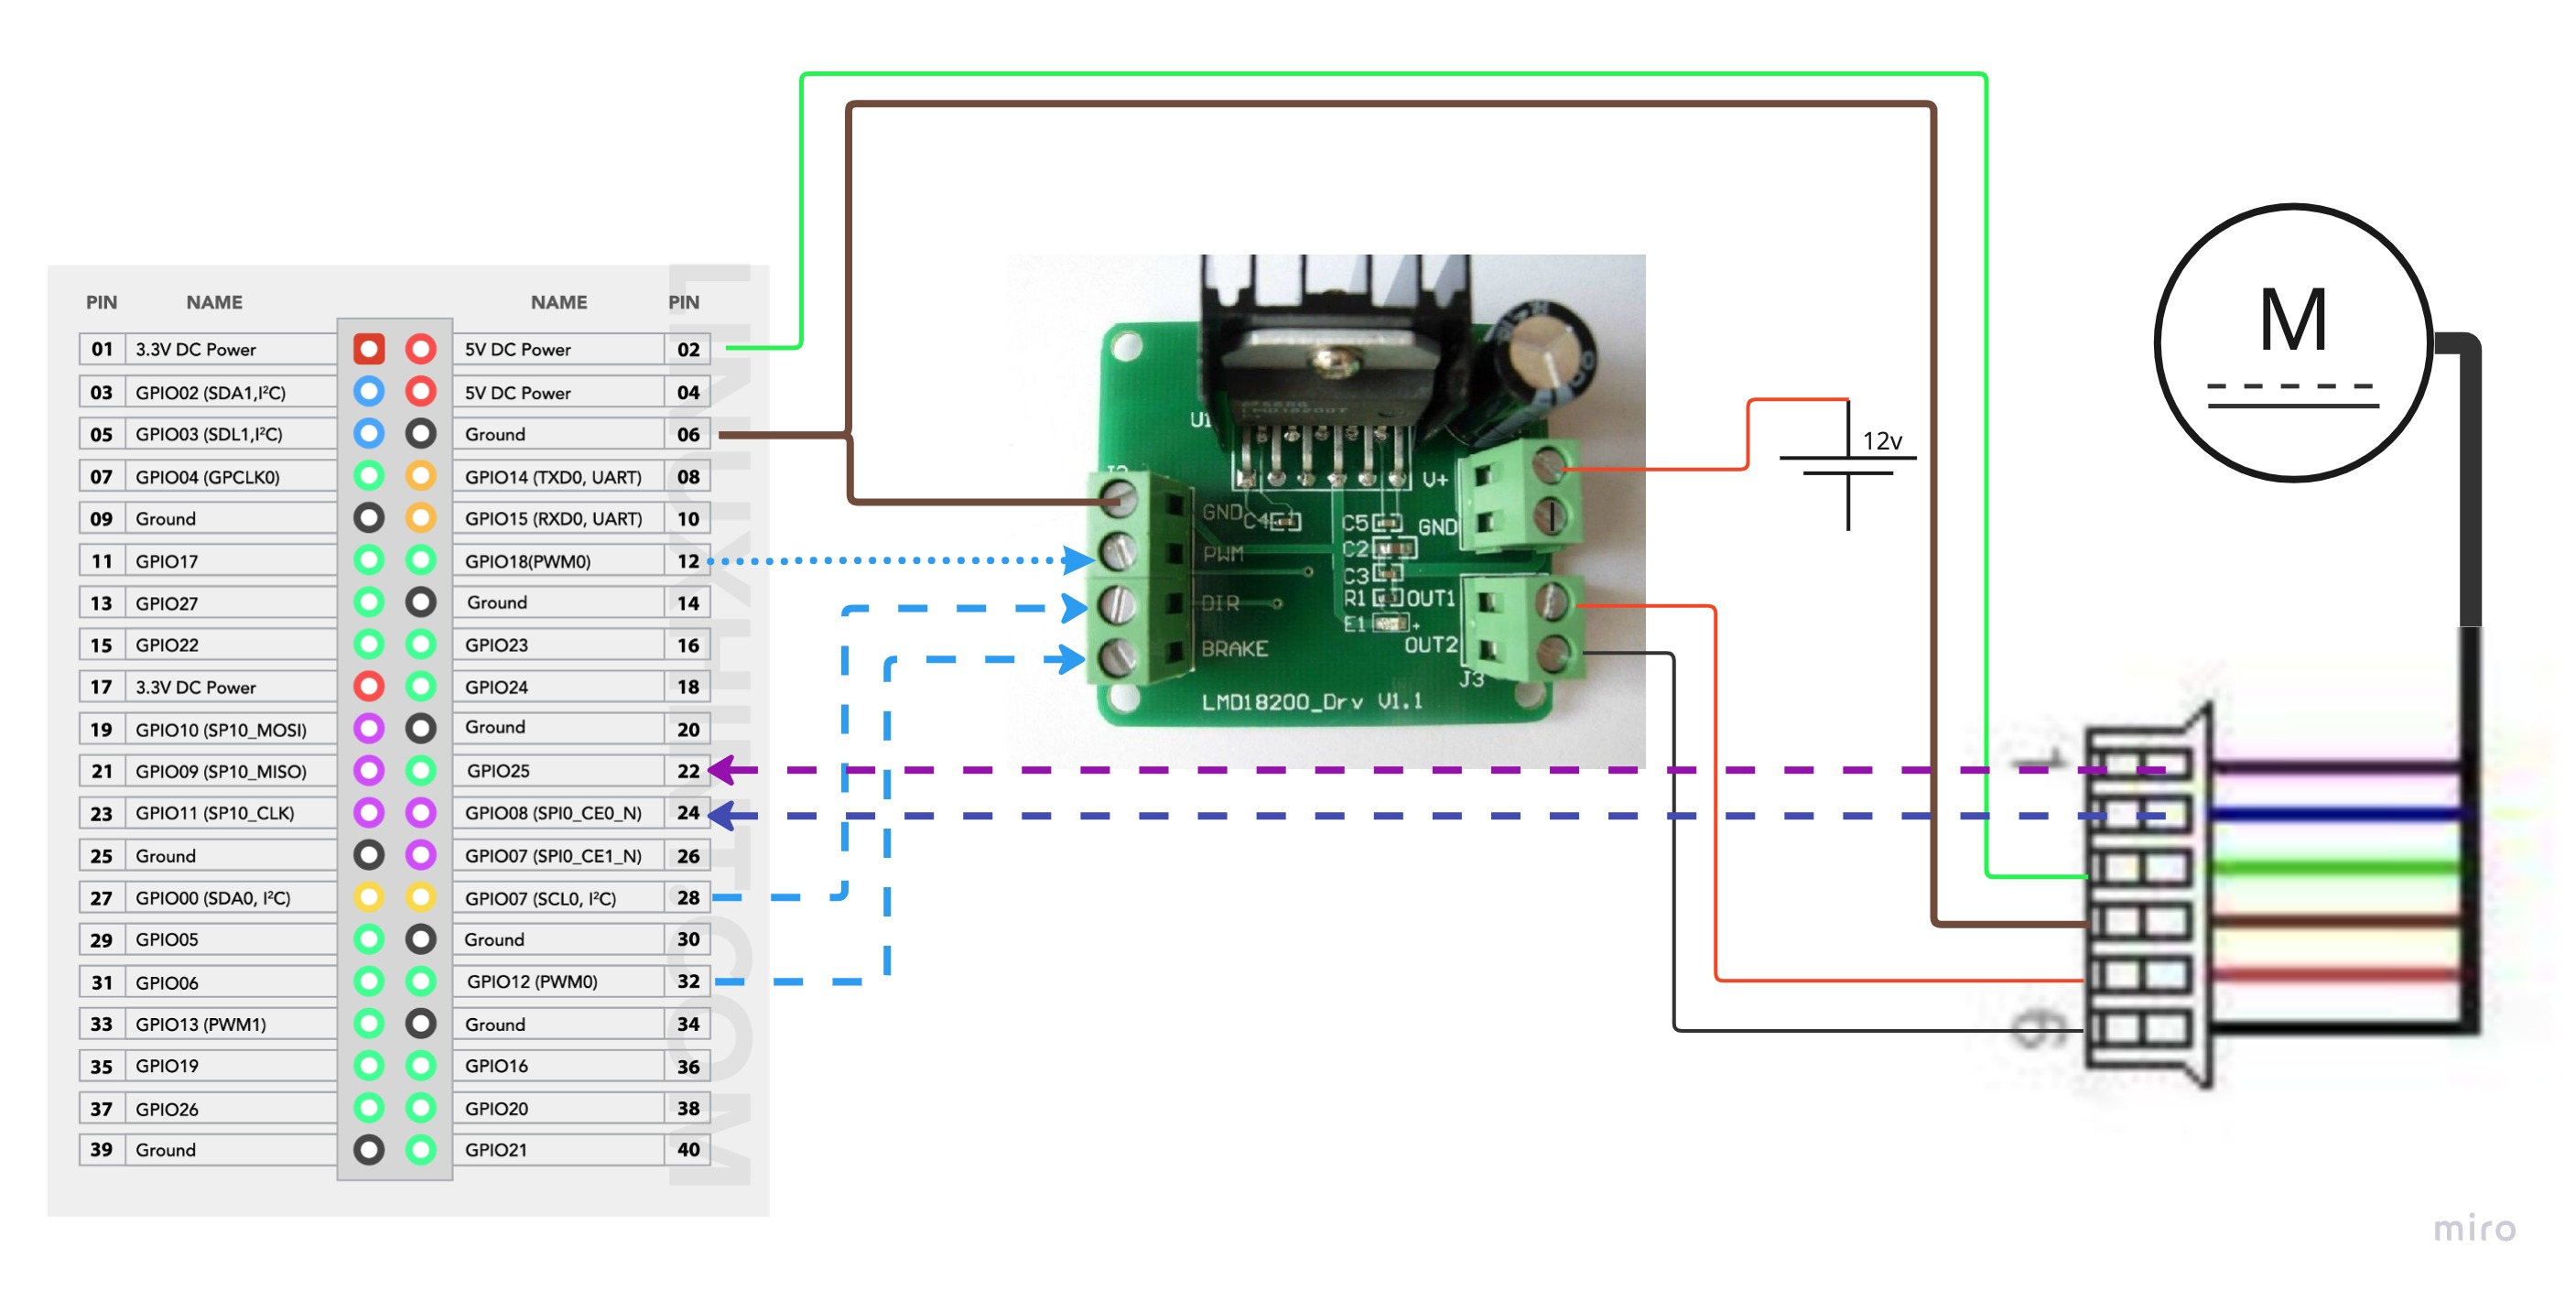
\includegraphics[scale = 0.15]{part/Proyecto_ejecutivo/memoria_constructiva/motor/img/connection diagram}
		\caption[Esquema de conexión del módulo de potencia.]{Esquema de conexión del módulo de potencia.\\Fuente: elaboración propia.}\label{fig:figure2}
\end{figure}